\documentclass{beamer}
\title % (optional, only for long titles)
{Marking Work}
%\subtitle{Evidence from India}
\author[Author, Anders] % (optional, for multiple authors)
{Andrei~Purice \and Alexandru~Tache}

\subject{Marking Supervisions}
\usetheme{Singapore}
\usepackage[latin1]{inputenc}
\usepackage{tikz}
\usetikzlibrary{shapes,arrows}
\begin{document}
  % Define block styles
  \tikzstyle{decision} = [diamond, draw, fill=blue!20, 
      text width=4.5em, text badly centered, node distance=3cm, inner sep=0pt]
  \tikzstyle{block} = [rectangle, draw, fill=blue!20, 
      text width=5em, text centered, rounded corners, minimum height=4em]
  \tikzstyle{line} = [draw, -latex']
  \tikzstyle{cloud} = [draw, ellipse,fill=red!20, node distance=3cm,
      minimum height=2em]
	%\frame{\titlepage}
	\begin{frame}
		\frametitle{Otter Handins}
    \framesubtitle{Supervising tool to organize, mark and store students work}
		%\framesubtitle{Supervising tool to organize, mark and store students work}
		\begin{center}	
		 
\includegraphics[height=7cm]{otter.jpg}
		\end{center}
    \end{frame}
	\begin{frame}
    	\frametitle{Managing supervisions is hard}
 
   	   	\begin{itemize}
   	   		\item Hard to organize and print the work from the students
          \item Work might not be submitted on time or in a good format
   	   		\item Parts of the work might get lost or overlooked
   	   		\item No easy way for a DoS to look at a students work
  	   	 \end{itemize}	   	 
  	\end{frame}
  	
    \begin{frame}
        \begin{tikzpicture}[node distance = 2cm, auto]
            % Place nodes
            \node [block] (bin) {Create bin};
            \node [cloud, left of=bin, node distance=3.5cm] (supervisor) {Supervisor};
            \node [cloud, right of=bin, node distance=4.3cm] (otter) {Through Deadlines};
            \node [block, below of=bin] (upload) {Upload Work};
            \node [block, below of=upload] (mark) {Mark Work};
            \node [block, below of=mark] (distribute) {Distribute Work};
            
            % Draw Edges
            \path [line] (bin) -- (upload);
            \path [line] (upload) -- (mark);
            \path [line] (mark) -- (distribute);
            
            \path [line, dashed] (supervisor) -- (bin);
            \path [line, dashed] (otter) -- (bin);
         
        \end{tikzpicture}
    \end{frame}
  	\begin{frame}
    	\frametitle{Our approach}
    	\begin{itemize}
        \item A bin is a place where students can throw in a supervision's work
    		\item Convert different work formats automatically to PDF 
    		\item Work is easily accessible anywhere, anytime, forever
    	\end{itemize}
    \end{frame}
    \begin{frame}
    	\frametitle{What it means for the student...}
    	\begin{itemize}
        
    		\item Submit work as either PDF, Text or scanned images
    		\item Students may select questions on their work
    		\begin{itemize}
    			\item Automatically using some special markup for the ones that are computer readable (PDF, Text)
    			\item Manually using a web interface we provide   			
        \end{itemize}
    	\end{itemize}    	
    \end{frame}
    {
      \setbeamercolor{frametitle}{fg=white, bg=black}
      \setbeamercolor{background canvas}{bg=black}
      \begin{frame}[plain]
        \frametitle{CamScanner}
        \makebox[\linewidth][c] {%
          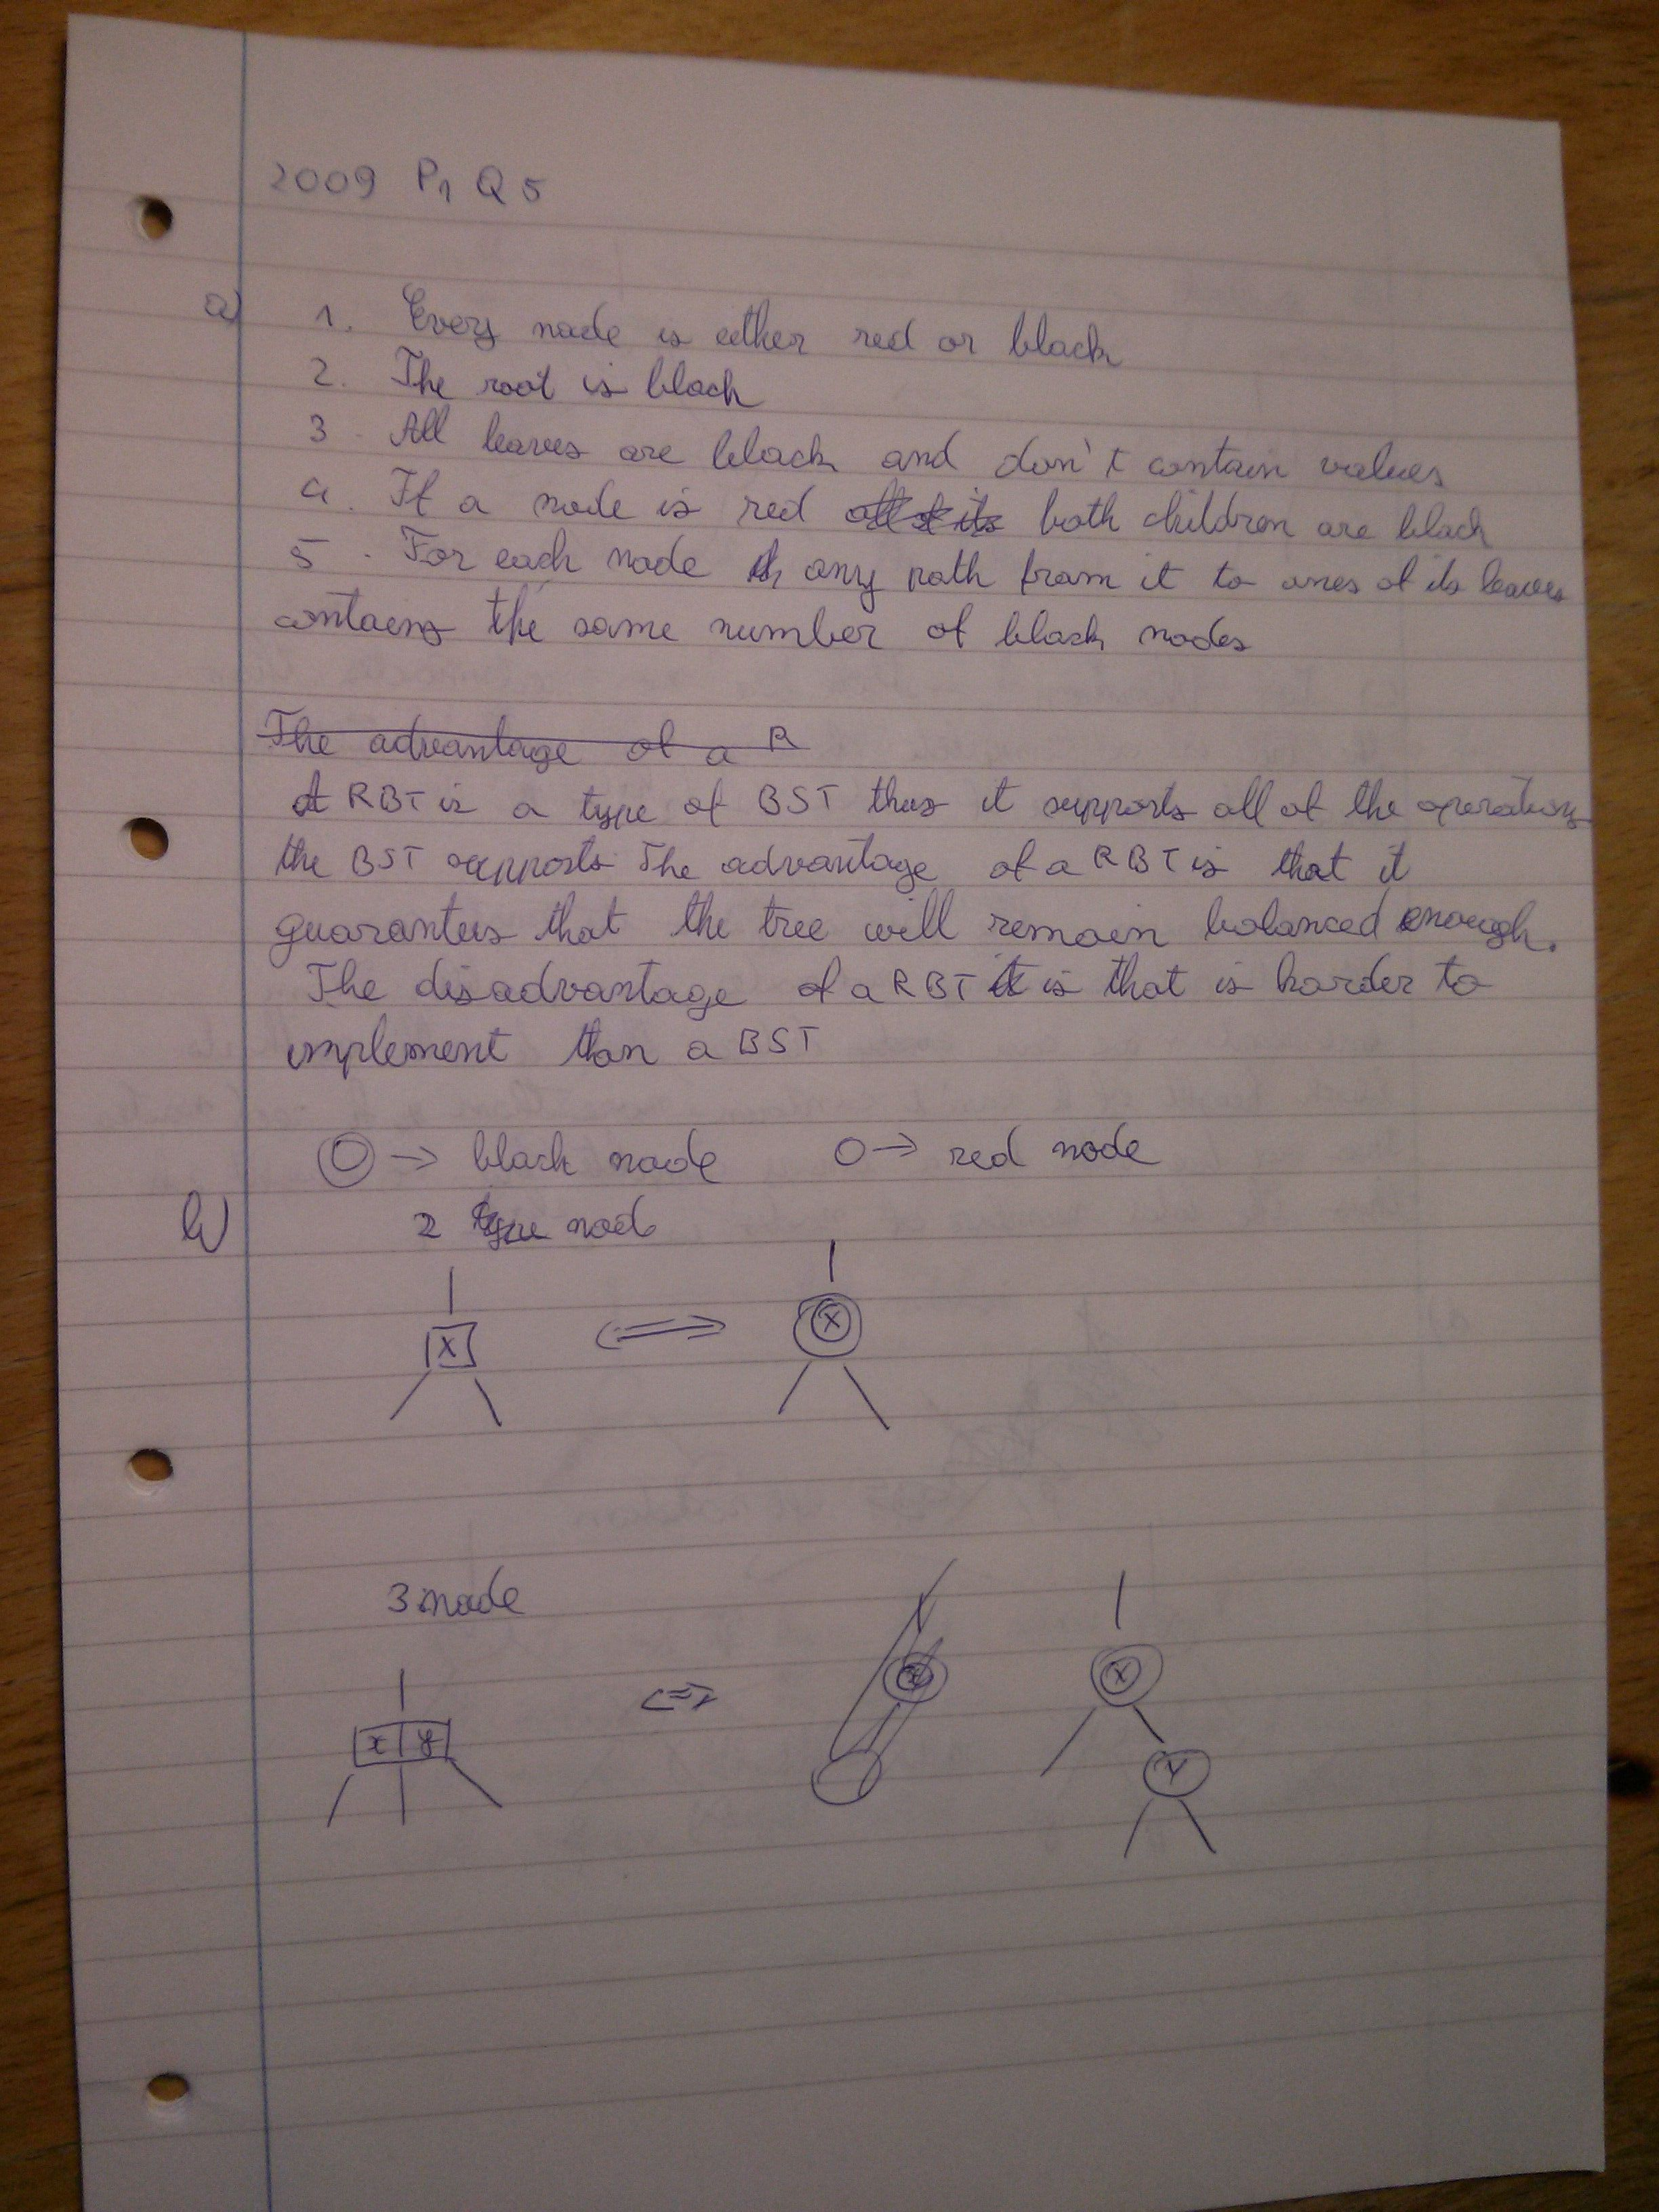
\includegraphics[height=4cm]{before.jpg}
          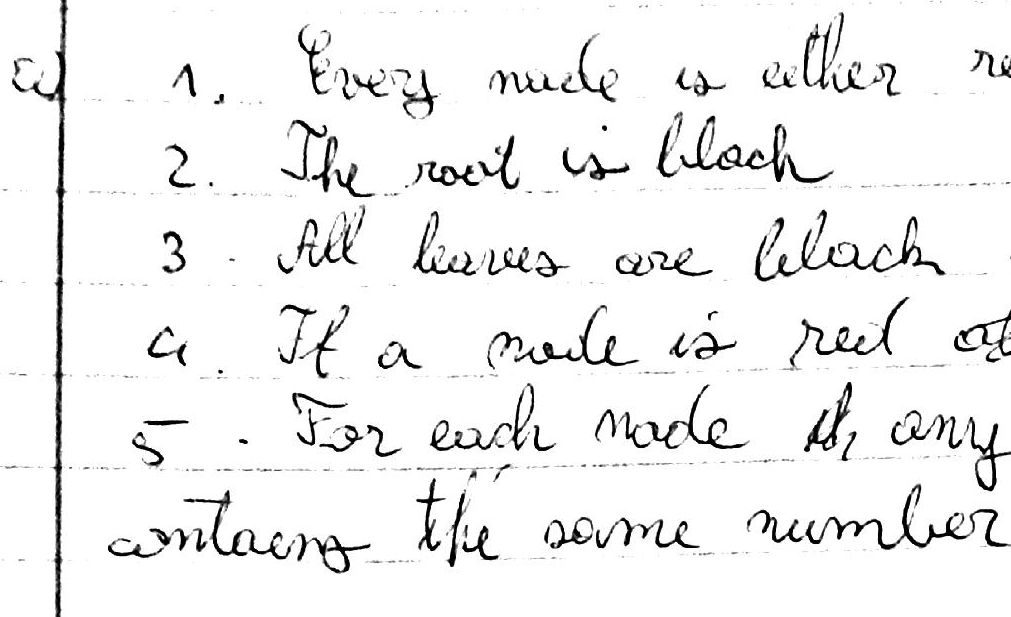
\includegraphics[height=4cm]{after.jpg}
        }  
      \end{frame}
    }
    \begin{frame}
    	\frametitle{...and for the supervisor}
    	\begin{itemize}
    		\item We provide PDFs with the work filter by student or by question
    		\item PDFs can be annotated with Xournal or other tools
    		\item We detect and store the changes on the PDFs.
    	\end{itemize}
    \end{frame}
    
    \begin{frame}
    	\frametitle{New ways to improve the supervision}
    	\begin{itemize}
    		\item Students can review their marked work before the supervision.
    		\item Peer marking.
    	\end{itemize}
    \end{frame}
    \begin{frame}
    	\frametitle{Thank You}
    \end{frame}
\end{document}